\documentclass{acmsiggraph}
\graphicspath{{../figures/}}
\usepackage{float}
\usepackage{amsmath, amsthm, amssymb}
\usepackage[linesnumbered,ruled,vlined]{algorithm2e}

\newcommand\mycommfont[1]{\footnotesize\ttfamily{#1}}
\SetCommentSty{mycommfont}

\title{Smoothed Local Histogram Filters \\
Project Report - Sparsity and Compressed Sensing}

\author{Maha ELBAYAD \\\texttt{maha.elbayad@student.ecp.fr}}
\pdfauthor{Maha ELBAYAD}

% User-generated keywords.

\keywords{Mode filters, Bilateral filter, Median filter, Local histogram}
\newcommand{\Gv}{G_{\mathit{\sigma_v}}}
\newcommand{\Gx}{G_{\mathit{\sigma_x}}}
\DeclareMathOperator\erf{erf}

\begin{document}

 % \teaser{
 %   \includegraphics[height=1.5in]{sampleteaser}
 %   \caption{Spring Training 2009, Peoria, AZ.}
 % }

\maketitle

\begin{abstract}

Local histograms filters exploit the information carried by the intensities distribution in the neighborhood of each pixel in order to shift those intensities according to a chosen scheme. These filters encompass some well known filters in the field of image processing: median, erosion, dilation..., as well as recent mode-based filters namely the closest and dominant mode.

In this project we will present and implement Kass and Solomon [2010] method to compute smooth local histograms, their derivatives and their integrals and then use those statistics to design the histogram filters. 
\end{abstract}

\keywordlist

\section{Introduction}
Local histograms are widely used in image processing for the useful amount they contain and the variety of filtering techniques they facilitate. However, histogram based filters are computationally expensive especially on large neighborhood and efficient algorithms are primordial to achieve good results at the required precision. The framework proposed by Kass and Solomon [2010] has the advantage of covering different filters and smoothly integrating the histogram-based computations in state of the art image processing techniques.

\section{Local histograms}
\subsection{Density estimation}
Instead of considering the traditional binned histogram we use kernel density estimation to approximate the distribution $f$ of the intensities $(I)$ in the considered neighborhood.

We will use the radial basis function as a smoothing kernel:
\[K(x) = \Gv(x) \equiv \exp\left(-\frac{x2}{2\sigma_v^2}\right)\]
Such kernel has the advantage of preserving the extrema of $f$ without introducing any further extrema in the smoothing process.

For a given pixel $p$, the estimated distribution is as follows:
\[\hat f_p(s) = \sum_i \Gv(I_{q_i}-s)W(p-q_i)\]
which we can rewrite as the convolution product:
\begin{equation}
\hat f_p(s) = \Gv(I_p - s) \otimes W\label{hist}
\end{equation}

$W$ is a weight matrix with unit sum that scatters the influence over the neighboring pixels $(q_i)_i$. If both $W$ and $K$ are unit box areas we'll end up with the bins histogram, instead we prefer to pair the intensities Gaussian kernel $\Gv$ with a spatial Gaussian kernel $\Gx$ so that the influence of the nearby pixels diminishes with distance. Generally for a Gaussian $\Gx$ we restrain the neighborhood to a square of size $2\sigma_x+1$.
\begin{figure}[H]
\centering
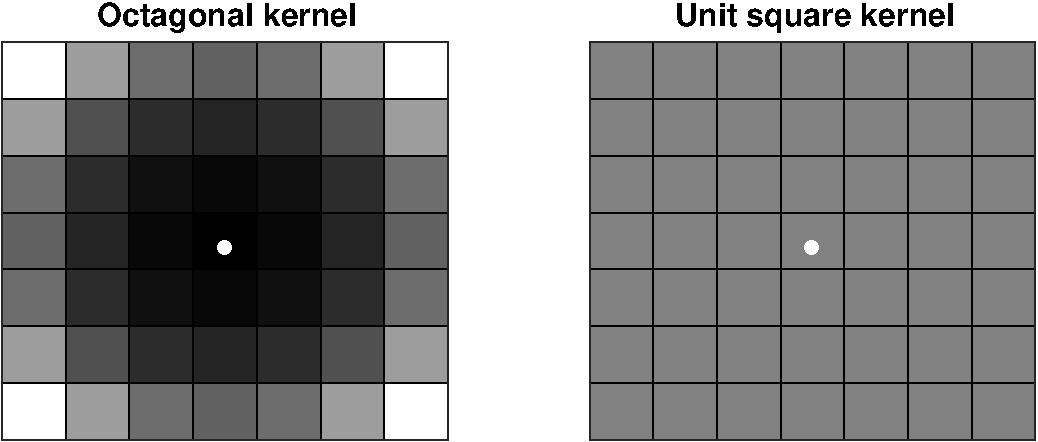
\includegraphics[width=6cm]{kernels}
\caption{Spatial kernels - $\sigma_x = 3$ }
\end{figure}
To sample the histogram shifts $(s_i)_{1\leq i\leq m}$, we use a frequency larger than the Nyquist frequency i.e for a Gaussian low pass filter of cut-off frequency $f_c = \frac{1}{2\pi\sigma}$, $m = f_{\text{sampling}}\geq f_{\text{Nyq}}=2f_c$.

\subsection{Derivative:}
The modes of the the histogram $f_p$ are an interesting feature to analyze: if $f_p$ has a single mode (local maxima) then the nearby pixels of $p$ might probably fall within the same population. Otherwise, the number of modes reflects the distinct populations in $p$'s neighborhood. To find the modes we compute the derivatives of $\hat f_p$ from \ref{hist}:
\begin{equation}
\begin{split}
\forall i\{1,..,m\},\: D_i(p) & = - \Gv'(I_p-s_i)\otimes W \\
       & = \frac{1}{\sigma_v^2}(I_p-s_i)K(I_p-s_i)\otimes W\\
\end{split}
\end{equation}
To locate a mode, we look for negative going zero crossings in $(D_i(p))_{1\leq i\leq m}$ between two consecutive samples $[D_i(p),\: D_{i+1}(p)]$ then with linear interpolation we approximate the mode's intensity:
\[s = s_i + \frac{D_i(p)}{D_i(p) - D_{i+1}(p)}(s_{i+1}-s_i)\]
Following the same steps we can approximate the antimodes (local minima) as the positive going zero crossings.
\begin{figure}[H]
\centering
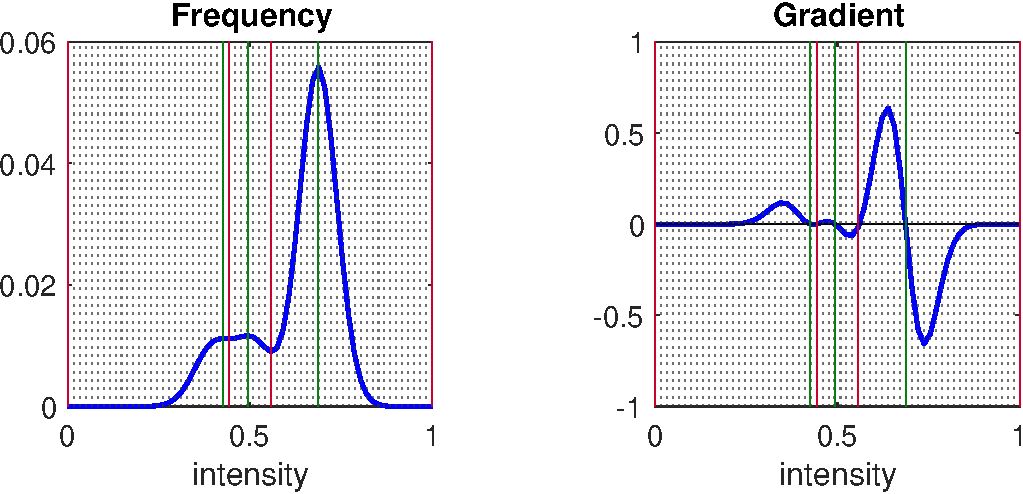
\includegraphics[width=9cm]{modes}
\caption{Histogram and its derivative with modes in green and antimodes in red for a given pixel}
\end{figure} 

\subsection{Integral:}
We can estimate the integrals of $f_p(s)$ as:
\[
R_p(s) = \int_{-\infty}^s \hat f_p(s) ds = \phi(I_p-s)\otimes W
\]
Sampled at shifts $(s_i)_{1\leq i\leq m}$:
\begin{equation}
R_i(p) = \phi(I_p-s_i)\otimes W
\end{equation}
Where for the Gaussian kernel $\Gv$:
\[\phi(z) = \sigma_v \sqrt{\frac{\pi}{2}} \left(1 + \erf\left(\frac{z}{\sigma_v\sqrt{2}}\right)\right)\]

\section{Histogram filters}
we will limit the scope of this project to 1D-histogram, filtering a single channel only. To process color images we map the input RGB image to HSV space, and then filter the Values channel $V$ before converting back to RGB.
\subsection{Morphological filters}
The morphological filters are a generalization of the rank filters, in case $W$ is the unit area. Those are non-linear local filters that sort the pixels in a neighborhood and select the ranked entry at $\lfloor \beta m\rfloor$, where m =$|$neighborhood$|$.

Generally, the morphological filter of order $\beta$ outputs the $\beta-$percentile of the intensities within the neighborhood. i.e.
\[\mathbb P(I\leq x) = \beta\]

The particular cases of $\beta = 0\%$ (erosion)
and $\beta = 100\%$ (dilation) are not affected by the scattered weights $W$, thus we modify the percentiles to $5\%$ and $95\%$ respectively. 

\begin{figure}[h]
\centering
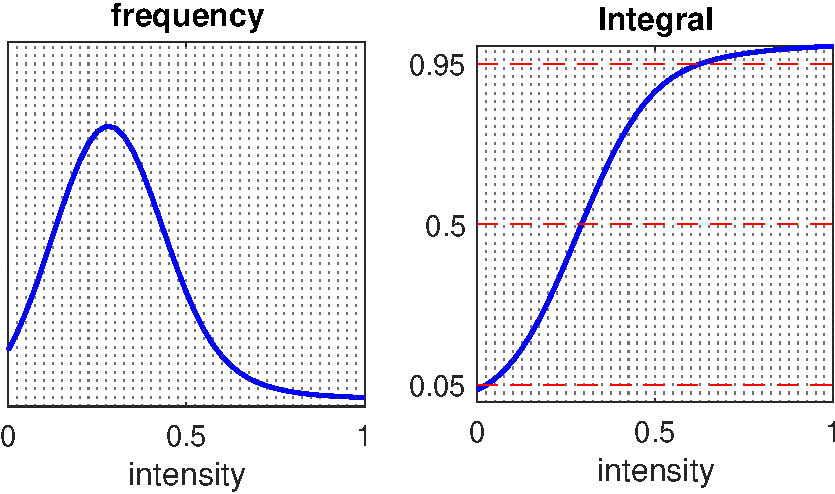
\includegraphics[width=8cm]{int}
\caption{Integral of the histogram and $\{5\%, 50\% , 95\%\}$ percentiles in red}
\end{figure}
The most popular rank filter is the median $(\beta = 50\%)$ which is particularly efficient and robust against impulse noise as can be seen in figure 4.
\begin{figure}[h]
\centering
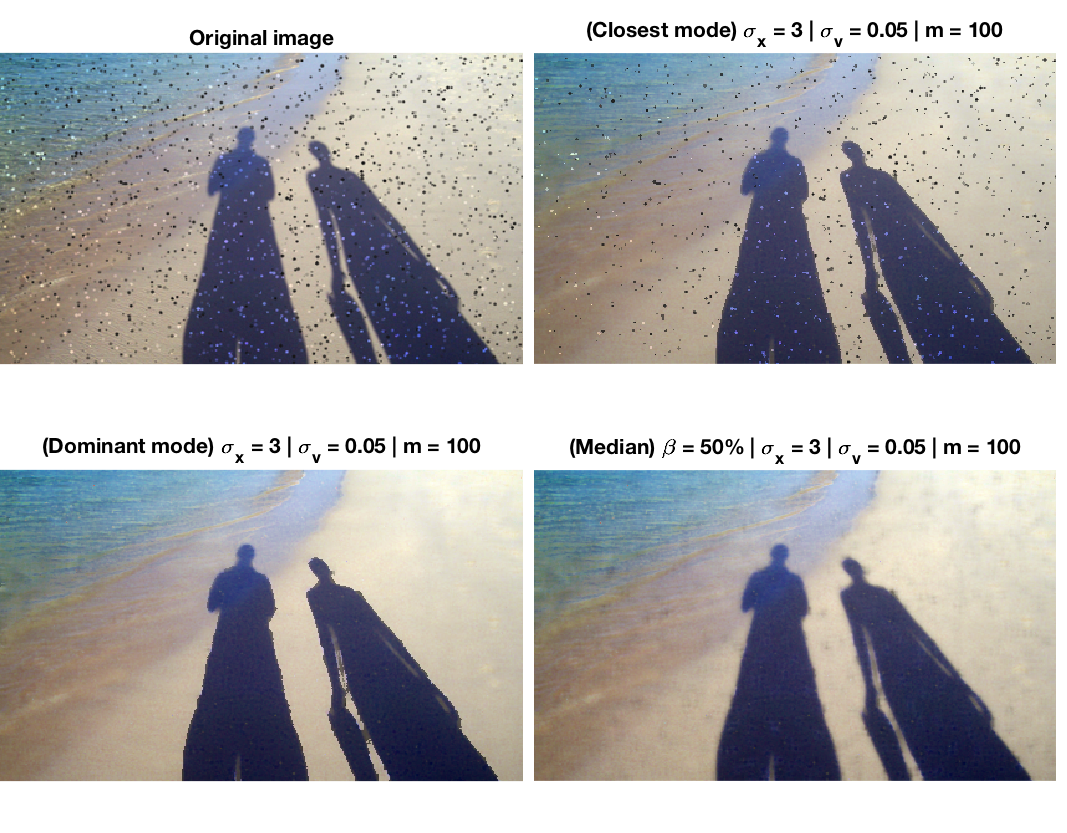
\includegraphics[width=9cm]{noisy}
\caption{Processing noisy image with different histogram filters}
\end{figure}

\subsection{Bilateral filter}
Similarly to the linear Gaussian convolution, the bilateral filter is defined as a weighted average of pixels. The difference is that the bilateral filter takes into account the variation of intensities to preserve edges. In terms of local histograms:
\[BF_p(s) = \frac{1}{Z}\sum_i\Gv(I_{q_i}-s)W(p-q_i).s\]
Where $Z$ is a normalization factor.

This can be written as a ratio of two convolutions:
\begin{equation}
BF_p(s) = \frac{(I_p\Gv(I_p-s))\otimes W}{\Gv\otimes W} 
\end{equation}
As in the previously introduced sampled signals we will linearly interpolate $BF(p)$ between $s_i$ and $s_{i+1}$ as follows:
\[BF(p) = s_i + \frac{\hat f_p(s_{i+1}) - \hat f_p(s_{i})}{s_{i+1} -s_i}(I_p-s_i)\]  

\subsection{Closest mode filter}
After identifying the modes in the local histogram we can assign the closest mode to the intensity of each input pixel, or alternatively choose the mode that we would reach by steepest ascent on the estimated density $\hat f_p$. This is equivalent to the convergence point of the iterative mean shift procedure introduced in Barash and Comaniciu [2004]. To determine the mode we first need to interpolate $D(I_p)$ from $(D_i(p))_{1\leq i\leq m}$ .i.e for $I_p\in[s_i,s_{i+1}]$:
\[D(I_p) = D_i(p) + \frac{D_{i+1}(p)-D_i(p)}{s_{i+1}-s_i}(I_p-s_i)\]
We select the first mode we encounter in the direction of the gradient, which means if $D(I_p)>0$ we pick the first mode larger than $I_p$, otherwise we select the last mode smaller than $I_p$.
\begin{figure}[h]
\centering
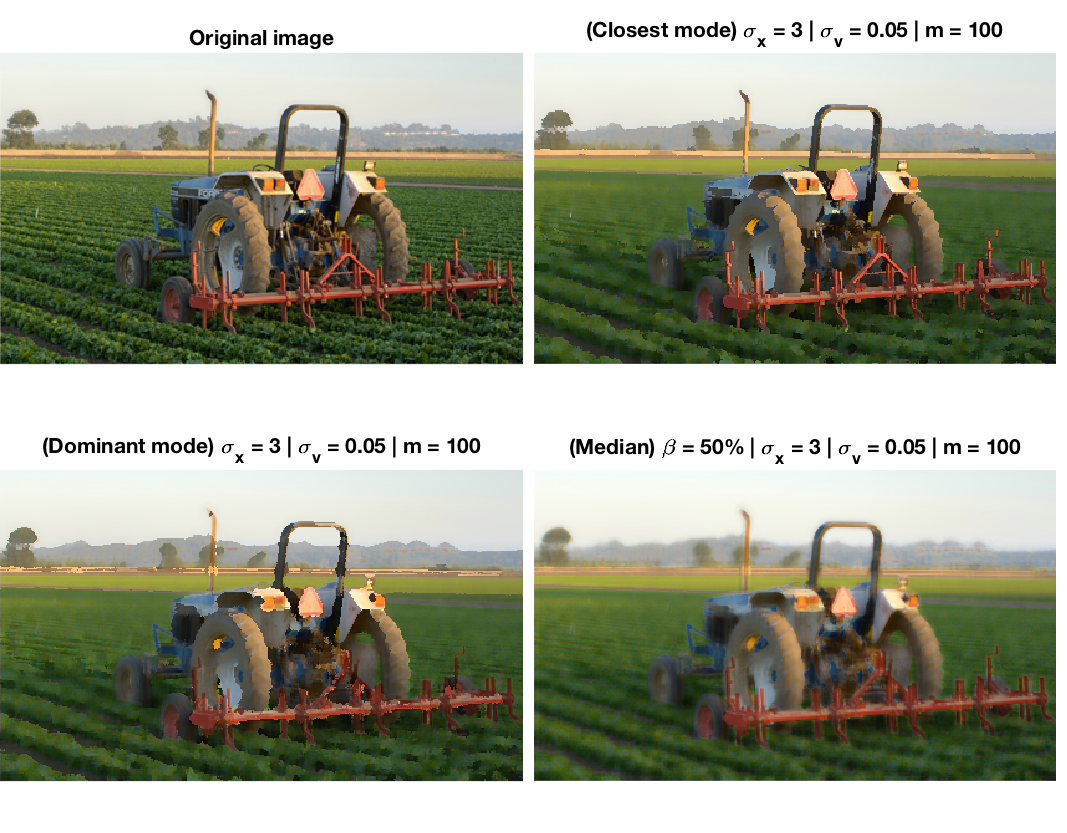
\includegraphics[width=9cm]{tractor.png}
\caption{Processing with different histogram filters}
\end{figure}

\subsection{Dominant mode filter}
Instead of choosing the closest mode to the pixel intensity, a more robust approach is to consider the mode with the largest population, the population size is reflected by the area between the two antimodes surrounding the considered mode i.e for $\mathit{m}_i\in(\mathit{a}_j,\mathit{a}_{j+1})$  
\[\begin{split}
A & = \int_{\mathit{a}_j}^{\mathit{a}_{j+1}}\hat f_p(s)ds\\
& = \left(\phi(I_p-\mathit{a}_{j+1}) - \phi(I_p-\mathit{a}_j) \right)\otimes W
\end{split}\]
\begin{figure}[H]
\centering
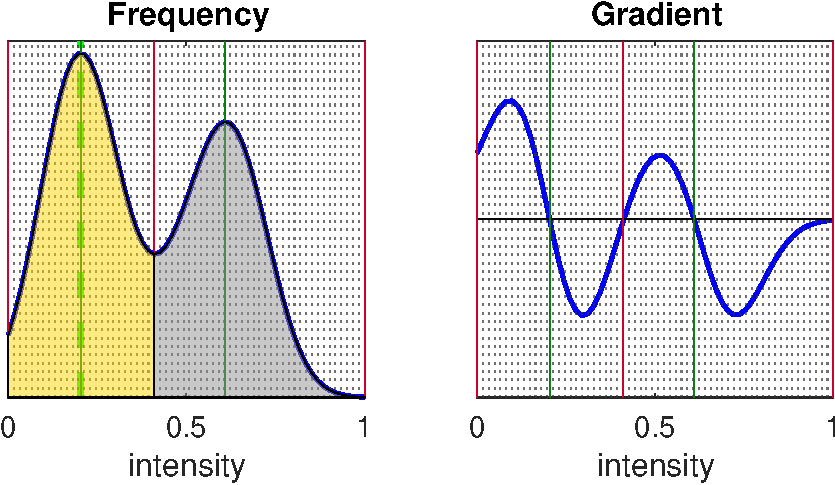
\includegraphics[width=7.5cm]{dominant_hist}
\caption{Dominant mode selection: modes in green and antimodes in red for a given pixel, the colored area represents the weight of each mode}
\end{figure}

\section{Applications in image processing}
\subsection{Image water-colorization}
A particular usage of morphological filters is  image stylization, in fact, 
Bousseau et al.[2007] consider the closing operator: erosion followed by dilation and opening operator : dilation followed by erosion, then define a new morphological filter : closing followed by opening.
\begin{figure}[H]
\centering
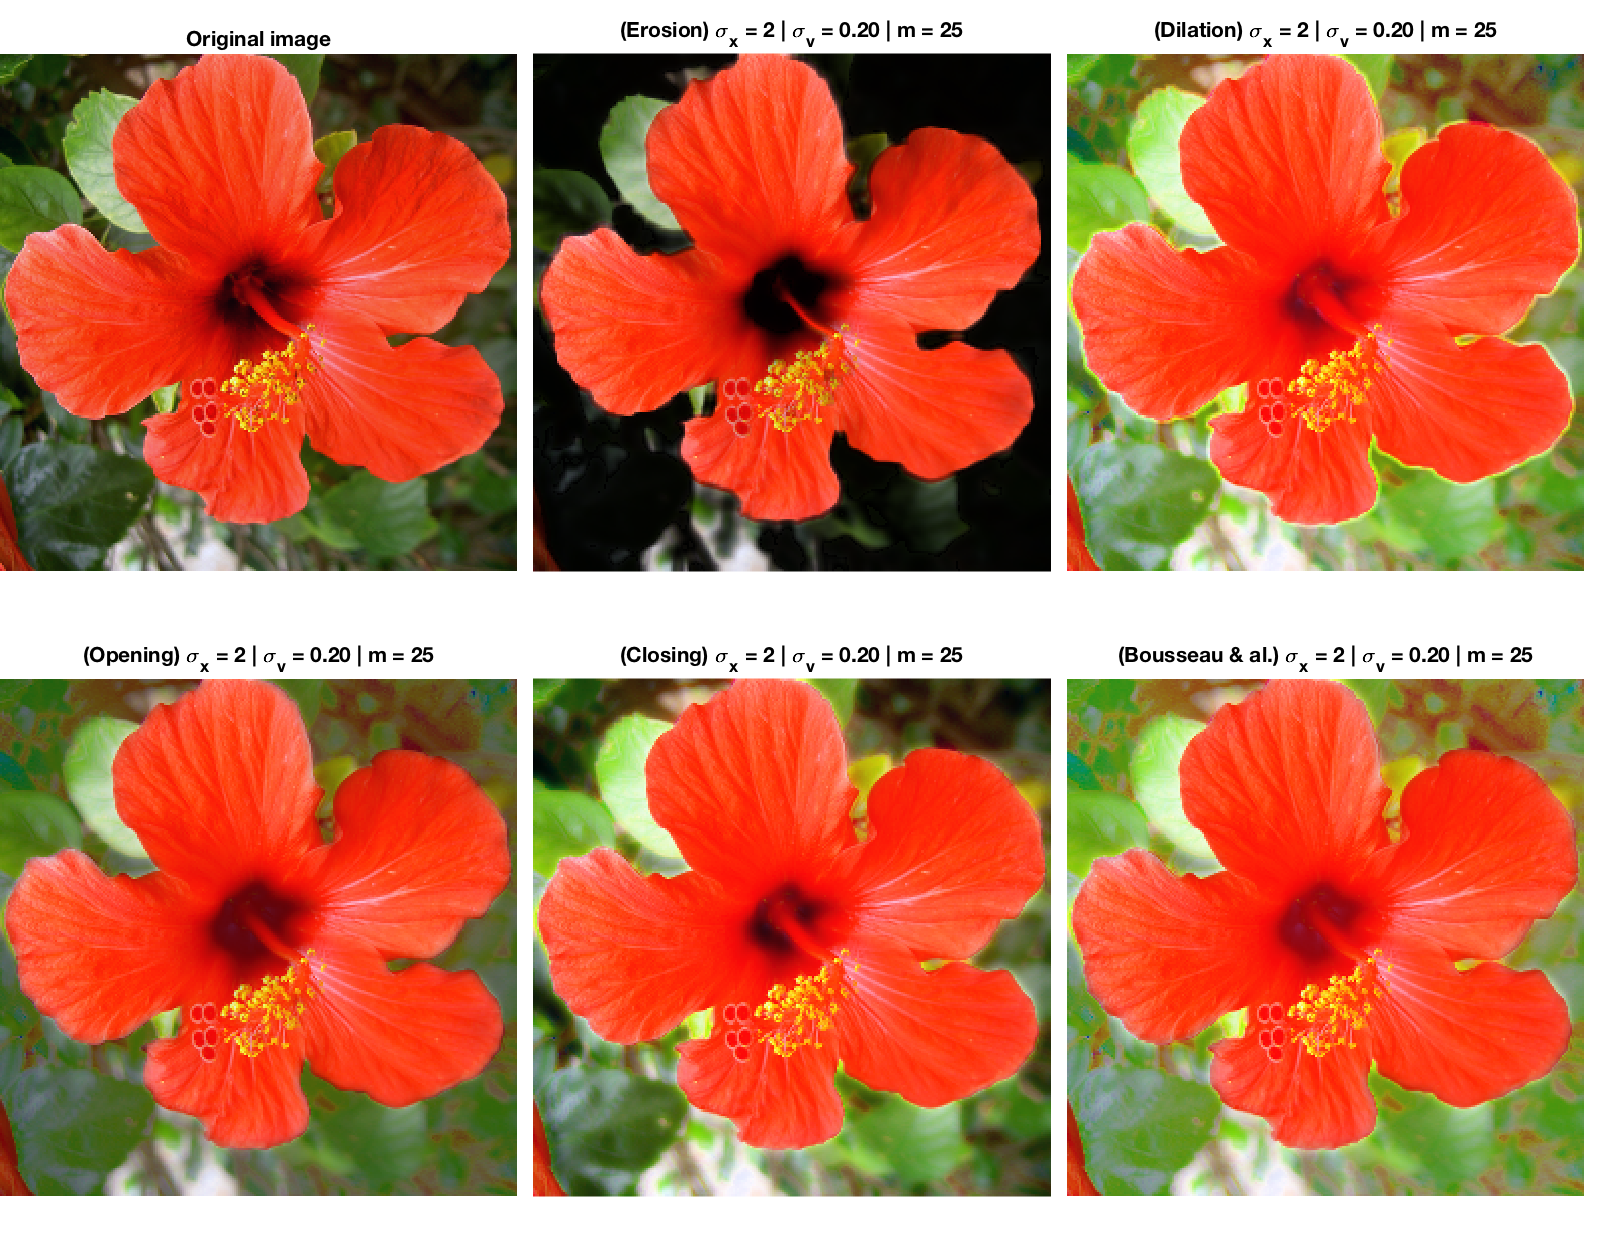
\includegraphics[width=9cm]{bousseau}
\caption{Applying morphological filters on local smooth histograms}
\end{figure}

\subsection{Detail enhancement}
\subsubsection{Selective Diffusion}
Detail enhancement algorithms rely on decomposing the input image into a piecewise-smooth base layer and a detail layer. The base layer is estimated with an edge-preserving smoothing filter such as the closest mode or the bilateral filters while the detail layer gathers what's left of the original image.
One way of extracting the base layer is selective diffusion. The method consists of blurring the edge-preserving filter and keep the closest intensity to the original image between the filter and its blurred version.
\begin{algorithm}
\DontPrintSemicolon
  \textbf{Inputs:} I : input image, $\eta$ : region size, $\sigma$ : blurring width \;
 \textbf{Initialization:}\;
 $D_0 = \text{filter}(I)$\;
 $\sigma_1 = \sigma$\;
 changes = $+\infty$\;
 i = 1\;
 \While{changes  $\neq 0$}{
  $B_i = D_{i-1}\otimes G(\sigma_i)$\;
  \tcc{local deviation of the unblurred version}
  $E_u = (D_{i-1} - I)^2\otimes G(\eta \sigma_i)$\;
  \tcc{local deviation of the blurred version}
  $E_b = (B_i - I)^2\otimes G(\eta \sigma_i)$\;
  $R = E_b / E_u$\;
  $B = \begin{cases}
  B_i \phantom{iiiiiiiiiiiiiiiiiiiiiiiiiiiiiiiiiii} R<.5\\
  2(R-\frac{1}{2})(D_{i-1}-B_i)+B_i \phantom{iiii} R\in[.5,1)\\
  D_{i-1} \phantom{iiiiiiiiiiiiiiiiiiiiiiiiiiiiiii} R\geq 1
  \end{cases}$\;
  i ++ \;
  $changes = numel(R<1)$\;
  $\sigma_i = \sqrt 2\sigma_i$\;
 }
\caption{Selective diffusion}
\end{algorithm}
\begin{figure}
\centering
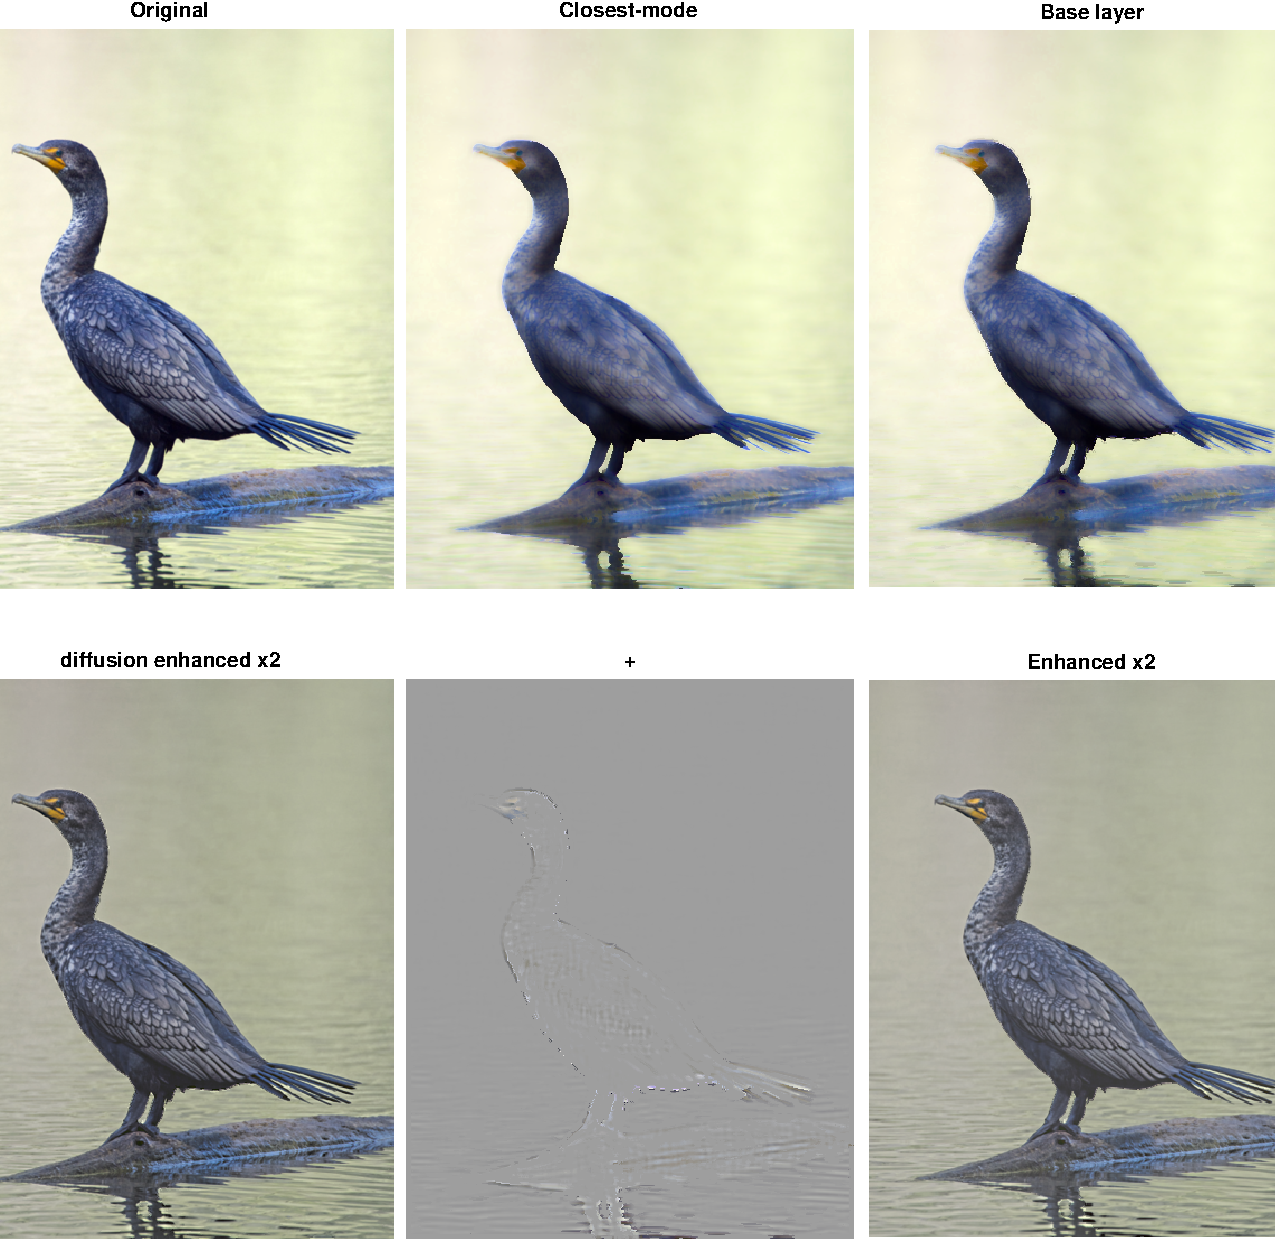
\includegraphics[width=9cm]{cormorant}
\caption{Detail enhancement with the closest mode filter \\$(\sigma_x=3,\sigma_v=.2,\sigma=\sigma_x,\eta=.2)$, converged after 8 iterations. The enhanced result equals the base layer plus twice the detail}
\end{figure}
The edges after filtering are sharp due to the discontinuities of the closest-mode filtering but after the diffusion step the edges seem softened and the result is more suitable as a base layer. Figure 8 illustrates the detail enhancement with and without diffusing after the closest mode filter, the middle figure if the second row shows the noisy details around the edges that we get rid off with diffusion.  

The bilateral filter is another interesting edge-preserving for detail enhancement, in figure 9 the enhanced image from the raw bilateral presents some artifacts namely halos and gradient reversals but after diffusion those artifacts were lessened.
\begin{figure}
\centering
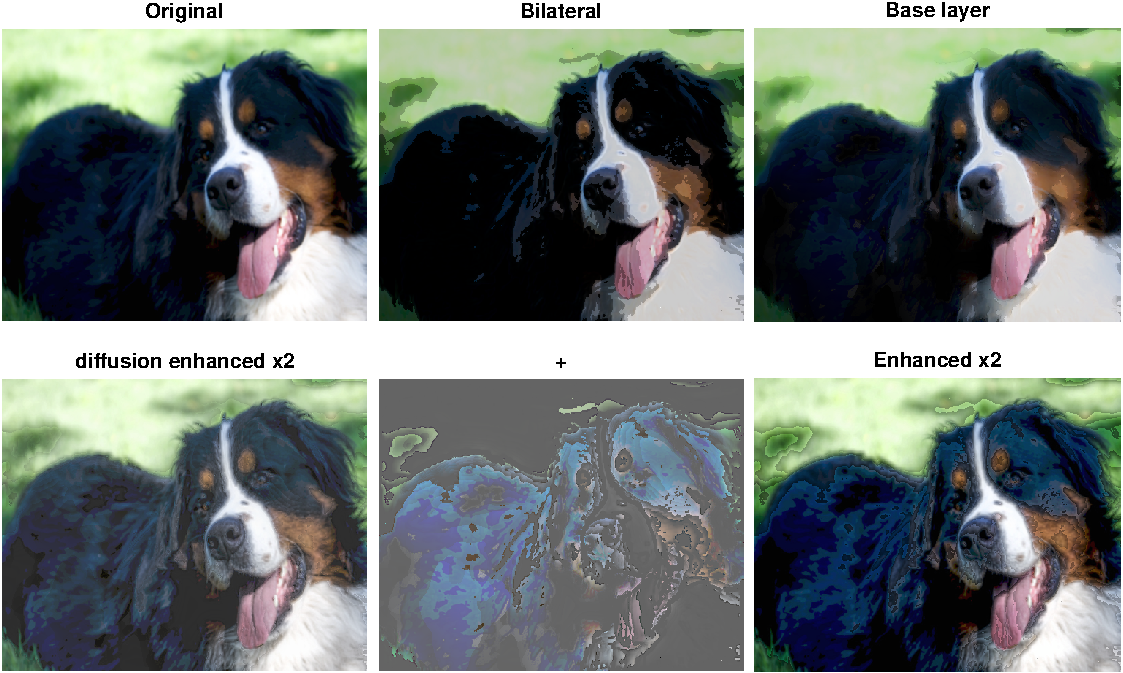
\includegraphics[width=9cm]{dog}
\caption{Detail enhancement with the bilateral filter \\$(\sigma_x=2,\sigma_v=.08,\sigma=\sigma_x,\eta=.2)$, converged after 8 iterations. The enhanced result equals the base layer plus twice the detail}
\end{figure}
\subsubsection{Multi-layer}
In the previous section we considered the detail layer to be the remaining of the input image after subtracting the detail layer. Alternatively we can construct a sequence of base layers if we iterate the same selective diffusion process .i.e decompose the detail layer at step i into a base layer $\mathcal B_i$ and a residual $\mathcal D_i$. After n steps we'll have:
\begin{equation}
I = \left(\sum\limits_{i=1}^n\mathcal B_i\right) + \mathcal D_n
\end{equation}
After each iteration we reduce the filter's values width $\sigma_v$ so that the decomposition is in terms of levels of contrast.

To achieve the results shown in figure 10 we choose $\sigma_v=( .1, .01, .0083)$ with $\sigma_x$ fixed at 8 and sampling $m =(10, 24, 24)$.
\begin{figure}[H]
\centering
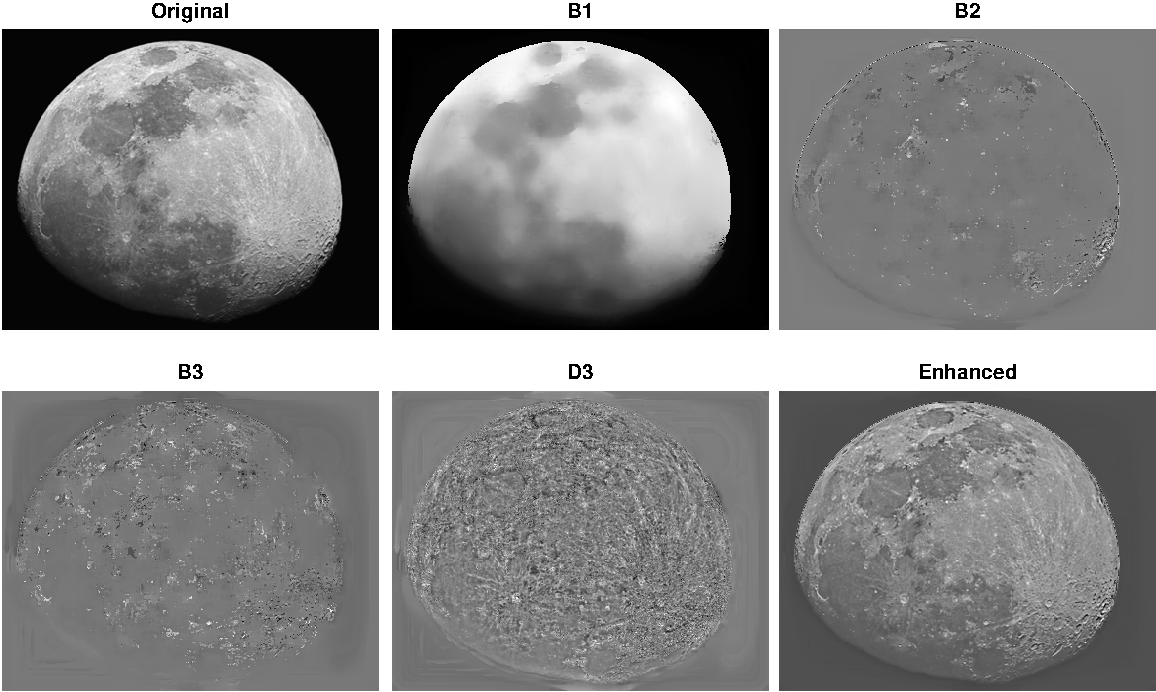
\includegraphics[width=9cm]{moon}
\caption{}
\end{figure}

\section{Conclusion}
This framework of histogram filters present a great opportunity to optimize different image processing techniques and the few applications above illustrate how robust the histogram-based computations can be.
\bibliographystyle{acmsiggraph}
\nocite{*}
\bibliography{template}
\end{document}
